% \subsection*{State of The Art}

% \begin{frame}[t]{Acoustic Echo Retrieval \hfill\faBook}
%     \begin{columns}[T,onlytextwidth]
%         \column{0.55\textwidth}
%             Estimating early (strong) reflections for microphones recordings, i.e.,
%             \begin{equation*}
%                 \{\contMic_i\}_i \longrightarrow \{ \tauir, \textcolor{gray}{\ampir} \}_{i,r}
%             \end{equation*}
%         \column{0.4\textwidth}
%             \begin{figure}
%                 \centering
%                 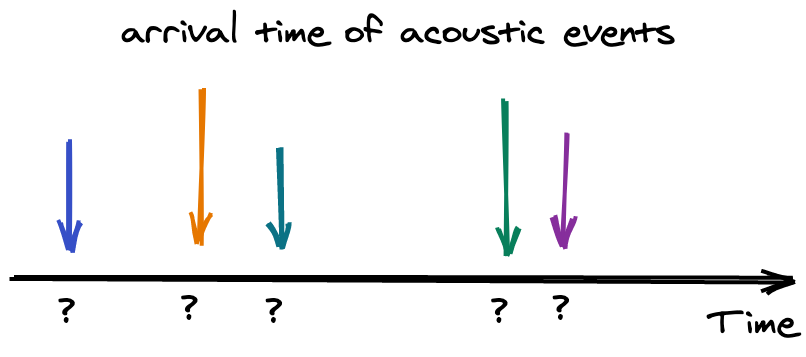
\includegraphics[width=\textwidth]{./figures/arrivals.png}
%             \end{figure}
%     \end{columns}

%     \vfill
%     \begin{columns}[T,onlytextwidth]
%         \column{0.48\textwidth}
%         \textbf{Scenarios:} the source signal is

%         \begin{center}
%             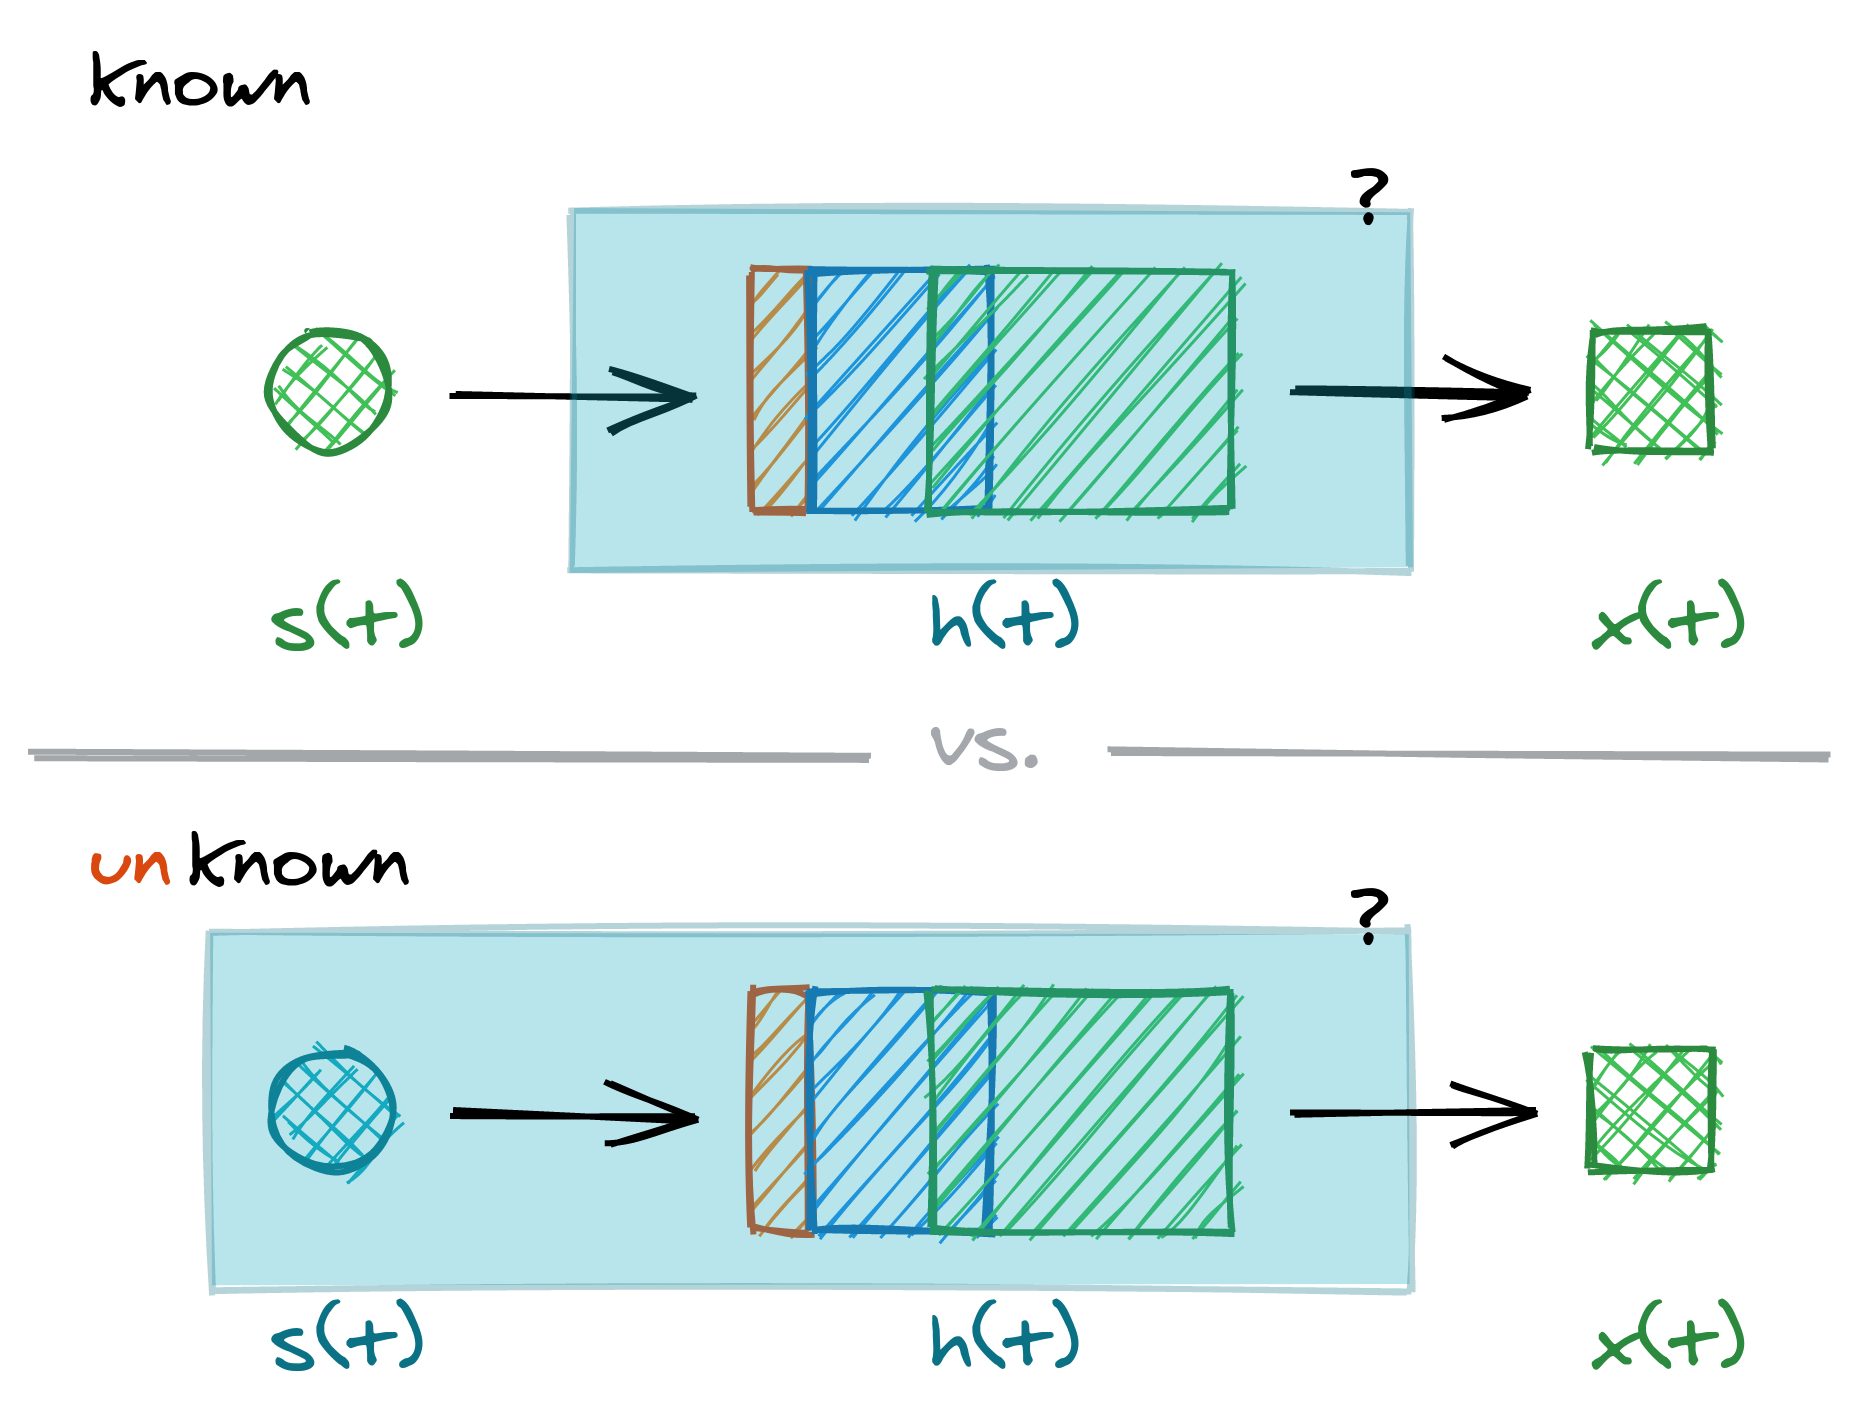
\includegraphics[width=.9\textwidth]{./figures/active-passive.png}
%         \end{center}

%         \only<4>{
%         \column{0.48\textwidth}
%         Active
%         \vspace{-2mm}
%         \begin{itemize}
%             \small
%             \item[\faEye] \textbf{non-blind} problem
%             \item[\faVolumeUp] \textbf{intrusive} or specific setups
%             % \item known emitted signal
%             % \item Time of Arrival (\textbf{TOA}s) accessible
%             % \\\hspace{.3em} $\implies$ \textbf{single} mic
%             \\\hspace{-1em}\addendum{\footnotesize \textbf{Application:} sonar, calibration, measurements, etc.}
%         \end{itemize}

%         \vspace{-5mm}
%         Passive
%         \vspace{-2mm}
%         \begin{itemize}
%             \small
%             \item[\faEyeSlash] \textbf{blind inverse} problem (harder)
%             \item[\faMicrophone] \textbf{passive} and more common setups
%             % \item \alert{un}knwon
%             % \item Time Difference of Arrivals (\textbf{TDOA}s) only
%             % \\\hspace{.3em} \textbf{multi-mic}
%             \\\hspace{-1em}\addendum{\footnotesize \textbf{Applications:} recording on smart speakers, laptop, etc.}
%         \end{itemize}
%         }

%         \only<5->{
%         \column{0.48\textwidth}
%         \centering
%         \textbf{Methods:} the estimation is
%         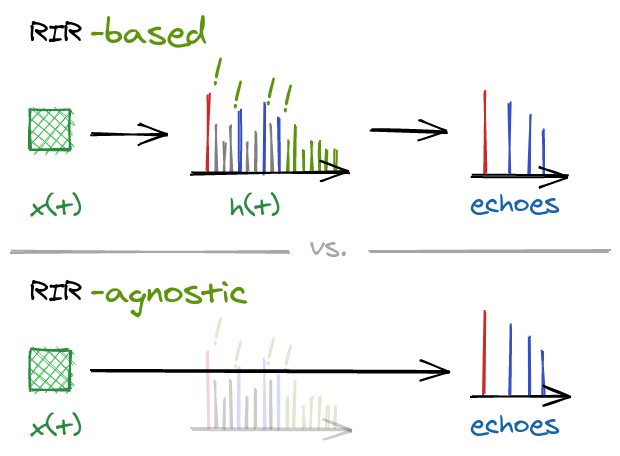
\includegraphics[width=.9\textwidth]{./figures/based-agnostic.png}
%         }
%     \end{columns}

%     \vfill
%     \textcolor{myred}{\textbf{Our case:} signal source and passive system of ($I$ microphones)}

% \end{frame}

% \begin{frame}[t]{\alert{Passive} Acoustic Echo Retrieval \hfill\faBook}

%         \vspace{.5em}
%         \begin{columns}[T,onlytextwidth] % align columns
%             \begin{column}{.48\textwidth}
%                 \textbf{RIR-\alert{based} approaches}
%             \end{column}
%             \begin{column}{.48\textwidth}
%                 \textbf{RIR-\alert{agnostic} approaches}
%             \end{column}%
%         \end{columns}

%         \vspace{.5em}
%         \begin{columns}[onlytextwidth] % align columns
%             \begin{column}{.48\textwidth}
%                 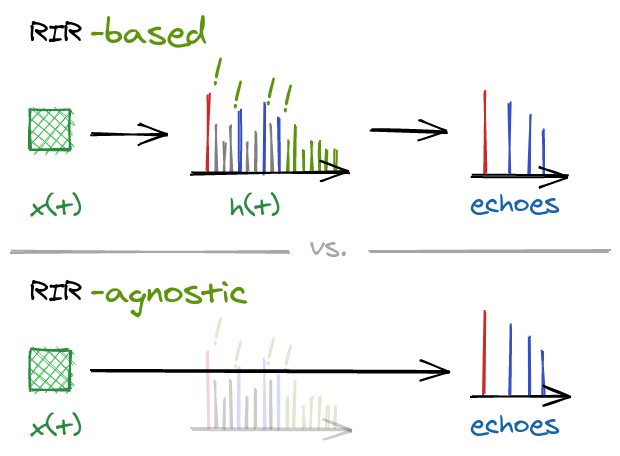
\includegraphics[trim={0 31em 0 7em},clip,width=.9\textwidth]{./figures/based-agnostic.png}
%             \end{column}
%             \begin{column}{.48\textwidth}
%                 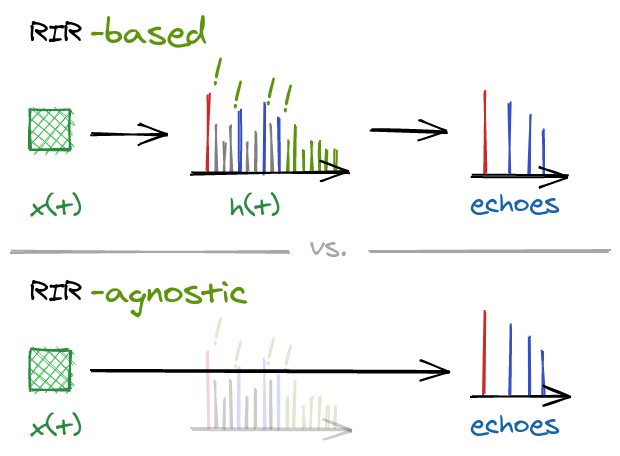
\includegraphics[trim={0 0 0 40em},clip,width=.9\textwidth]{./figures/based-agnostic.png}
%             \end{column}%
%         \end{columns}

%         \vspace{.5em}
%         \begin{columns}[T,onlytextwidth] % align columns
%             \begin{column}{.48\textwidth}
%                 \small
%                 \begin{enumerate}
%                     \item ``BCE''\footnotemark[1] problem $\implies$ RIRs
%                     \item Peak picking $\implies$ Echoes
%                 \end{enumerate}
%             \end{column}
%             \begin{column}{.48\textwidth}
%                 \small
%                 \begin{enumerate}
%                     \item Direct off-grid estimation of $\set{\tauir, \ampir}$
%                     e.g., with maximum-likelihood
%                     % \\\textcolor{gray}{(+ \small direction of arrivals can be used instead)}
%                 \end{enumerate}
%             \end{column}%
%         \end{columns}

%         \vspace{1em}
%         \begin{columns}[T,onlytextwidth] % align columns
%             \column{.48\textwidth}
%                 \small
%                 \begin{itemize}
%                     \item[\cmark] \pro{BCE is well and known studied}
%                     \item[\cmark] \pro{it is the state of the art}
%                     \\{\scriptsize~\cite{crocco2016estimation}}
%                     \item[\cmark] \pro{reasonably good for some application}
%                 \end{itemize}
%             \column{.48\textwidth}
%                 \small
%                 \begin{itemize}
%                     \item[\cmark] \pro{No full RIRs \& no peak picking}
%                     \begin{itemize}
%                         \item lower complexity
%                         \item less hyperparameters
%                     \end{itemize}
%                     \item[\cmark] \pro{Echo properties are respected}
%                     \\\addendum{\footnotesize e.g. Sparsity, Non-negativity}
%                     \end{itemize}
%         \end{columns}

%         \vspace{1em}
%         \begin{columns}[T,onlytextwidth] % align columns
%             \column{.48\textwidth}
%                 \small
%                 \begin{itemize}
%                     \item[\xmark] \con{Full RIRs need to be estimated}
%                     \item[\xmark] \con{Peak picking has hyperparameters}
%                     \item[\xmark] \con{Issues due to \textit{on-grid} estimation}
%                     \\[\footnotesize \faReply~next topic]
%                 \end{itemize}
%             \column{.48\textwidth}
%                 \small
%                 \begin{itemize}
%                     \item[\xmark] \con{exploratory \faWpexplorer}
%                     \\\addendum{no standard solver, few works on audio}
%                     % \item[\xmark] \con{no ``simple'' implementation}
%                     % \\\addendum{not standard math of BCE}
%                 \end{itemize}
%         \end{columns}

%     \footnotetext[1]{Blind Channel Estimation}

% \end{frame}

% \begin{frame}{Limitations \& bottleneck  \hfill\faBook}

%     \begin{block}{\faExclamationCircle~ Echoes are not necessarely ``on-grid''}

%         \vspace{-2mm}
%         \begin{itemize}
%             \item Sparsity and non-negativity not true ``on grid''
%             % We measure filters, not diracs

%             \item \emph{Body guard} effect \cite{duval2017sparse}
%             \begin{itemize}
%                 \item[$\rightarrow$] low recall $\implies$ low accuracy % (2 echoes instead of 1)
%                 \item[$\rightarrow$] slow convergence % bouncing between 2 echoes
%             \end{itemize}
%             \item Pick Picking
%             \begin{itemize}
%                 \item[$\rightarrow$] manually tuned / corrected
%             \end{itemize}
%         \end{itemize}
%     \end{block}

%     \begin{columns}[onlytextwidth]
%         \column{0.60\textwidth}

%         \begin{block}{How about higher sampling rate $F_s$?}

%             \vspace{-2mm}
%             \begin{itemize}
%                 \item[$\rightarrow$] Increase Precision
%             \end{itemize}
%         \end{block}

%         \begin{block}{But, computational bottleneck!}

%             \vspace{-2mm}
%             \begin{itemize}
%                 \item Bigger vectors and matrices
%                 \begin{itemize}
%                     \item[$\longrightarrow$] memory usage
%                 \end{itemize}
%                 \item the higher the sampling frequency
%                 \begin{itemize}
%                     \item[$\longrightarrow$] more ill-conditioned
%                 \end{itemize}
%             \end{itemize}
%         \end{block}

%         \column{0.38\textwidth}
%         \begin{center}
%             \textcolor{myred}{\textbf{How to address this?}}
%         \end{center}
%         \begin{mycontriblock}
%             RIR-agnostic + off-grid
%             \begin{enumerate}
%                 \item Deep Neural Network
%                 \item Continuous Dictionary
%             \end{enumerate}
%         \end{mycontriblock}

%     \end{columns}

%     \begin{textblock*}{40mm}(80mm,15mm)
%         \includegraphics<1->[width=\columnwidth]{figures/bodyguard.png}
%     \end{textblock*}

% \end{frame}

% \subsection{\lantern}

% \begin{frame}{Proposed approach: learning-based \& off-grid \hfill\faBrain}

%     % \textbf{Recall}: AER $\Leftrightarrow$ $\{\contMic_i\}_i \overset{?}{\longrightarrow} \{ \tauir, \textcolor{black!20}{\ampir} \}_{i,r}$
%     \begin{mydefblock}{Idea: (Deep) Learning-based AER}
%         \begin{enumerate}
%             \item Use \alert{virtually} supervised deep learning models
%             \item Estimate first echo (simple but important)
%             \item Only 2 microphones
%         \end{enumerate}
%     \end{mydefblock}

%     \vfill
%     \textbf{Motivations:}
%     \begin{itemize}
%         \item This \textit{direct} mapping is difficult, the \textit{inverse} ``is not''
%         \\$\rightarrow$ acoustic simulators:
%             $\text{mic/src/room geometry}
%             \; \longrightarrow \;
%             \set{\tauir,\ampir}, \; \contRIR_i, \quad \contMic_i$
%         \item Acoustic simulator are ``simple'', versatile and fast
%         \\$\to$ many data
%         \item This approach is successful in \textit{Sound Source Localization}
%         \\$\to$ position is related to echoes
%         \\{\small\cite{kataria2017hearing,nguyen2018autonomous,perotin2019regression} \textcolor{myred}{\faExclamationTriangle~Not only DNN}}
%     \end{itemize}

% \end{frame}

% \begin{frame}{Proposed approache: models \hfill\faBrain}

%     \begin{columns}[T,onlytextwidth]
%         \column{0.48\textwidth}
%         \textbf{Inputs:}
%         {\small Interchannel level and phase difference features\footnotemark[1] from
%             \[ \footnotesize
%             R[f] = \timeavg \frac{X_2[f,t]}{X_1[f,t]}
%             \approx \timeavg \frac{H_2[f]\alert{S[f,t]}}{H_1[f]\alert{S[f,t]}}
%             \]
%             \\$\approx$ the relative transfer function
%             \\$\to$ remove source dependency
%         }

%         \column{0.48\textwidth}
%         \textbf{Output:} {\small Inter and intra arrival delays}
%         \begin{columns}
%             \column{0.60\textwidth}
%             \includegraphics<1>[width=\textwidth]{figures/lantern_rir_tdoa1(1).png}%
%             \includegraphics<2>[width=\textwidth]{figures/lantern_rir_tdoa1(2).png}%
%             \includegraphics<3->[width=\textwidth]{figures/lantern_rir_tdoa1(3).png}%
%             \column{0.45\textwidth}
%             \footnotesize
%             \centering
%             4 TOA
%             \\$\downarrow$
%             \\3 Time \alert{Difference} of Arrivals (\alert{\textbf{TDOAs}})\footnotemark[1]
%         \end{columns}
%         \begin{center}
%             \small
%             \textbf{HP:} first $\Leftrightarrow$ strongest echo
%         \end{center}
%     \end{columns}

%     \pause[4]
%     \vfill
%     \begin{itemize}
%         \item Architecture: $\MLP$, $\CNN$~{\footnotesize\cite{chakrabarty2017broadband,nguyen2018autonomous}}
%         \item Loss Function:
%         \begin{enumerate}
%             \item RMSE (Multi-label regression) $\to$ TDOAs
%             \item Gaussian log-likelihood $\to \kbrace{\mu_\tau, \sigma^2_\tau} \;\forall \tau \in$ TDOAs \hspace{1em}\tikzmark{CNN}\tikzmark{CNNtop}
%             \item Student log-likelihood $\to \kbrace{\mu_\tau, \lambda_\tau, \nu_\tau} \;\forall \tau \in$ TDOAs \tikzmark{CNNbot}
%         \end{enumerate}

%         \pause[6]
%         \item Data:
%         \begin{itemize}
%             \item Virtually-supervised learning (= data from acoustic simulator)
%             \item white-noise as source signal + noise
%             \item 2 microphone in close-surface scenario
%         \end{itemize}
%     \end{itemize}

%     \visible<5->{
%     \begin{tikzpicture}[overlay, remember picture]
%         \node[anchor=base] (a) at (pic cs:CNNtop) {\vphantom{h}}; % push the mark to the top of the line (ie including ascenders)
%         \node[anchor=base] (b) at (pic cs:CNNbot) {\vphantom{g}}; % push the mark to the bottom of the line (ie including descenders)
%         \draw [decoration={brace,amplitude=0.35em},decorate,thick,gray]
%             (a.north -| {pic cs:CNN}) -- node[right,inner sep=1em] {
%                 \small \parbox{12em}{Good for data fusion\\Similar to \textbf{MDN}\\~{\footnotesize\cite{bishop1994mixture}}}
%                 } (b.south -| {pic cs:CNN});
%     \end{tikzpicture}
%     }

%     \visible<1->{
%         \footnotetext[1]{\tiny $\mathtt{ILD} = \log\kvbar{R}$, $\mathtt{IPD} = \arg{R/\kvbar{R}}$}
%     }

% \end{frame}

% \begin{frame}{\faFlask~Experimental results \hfill\faBrain}

%     \vspace{2mm}
%     \begin{mycontriblock}
%         \textbf{Proposed Method:} $\MLP$, $\CNN$, $\CNNn$, $\CNNt$
%     \end{mycontriblock}
%     \begin{mysotablock}
%         \textbf{Baseline:} $\GCCPHAT${\tiny~\cite{knapp1976generalized}}
%     \end{mysotablock}

%     \textbf{Metrics:} normalized RMSE (0 = best fit, 1 = random fit)

%     % \vspace{2mm}
%     % \begin{columns}[T,onlytextwidth]

%     %     \column{0.32\textwidth}
%     %     Are better than baseline?
%     %     \\\addendum{\footnotesize only TDOA on direct path}
%     %     \\\hspace{.3em}$\to$ yes \cmark

%     %     \column{0.32\textwidth}
%     %     Echoes' \alert{TDOAs}?
%     %     \\\hspace{.3em}$\to$ yes \cmark
%     %     \\\hspace{.3em}$\to$ CNN better than MLP

%     %     \column{0.32\textwidth}
%     %     Are robust to noise?
%     %     \\\hspace{.3em}$\to$ yes \cmark
%     %     \\\hspace{.3em}$\to$ \CNNn/\CNNt better than \CNN

%     % \end{columns}

%     \begin{center}
%         \includegraphics<1>[trim={0 30 0 0},clip,height=0.33\textwidth]{figures/lantern_snr1.pdf}%
%         \includegraphics<2>[trim={0 30 0 0},clip,height=0.33\textwidth]{figures/lantern_snr2.pdf}%
%         \includegraphics<3>[trim={0 30 0 0},clip,height=0.33\textwidth]{figures/lantern_snr3.pdf}%
%         \includegraphics<4->[trim={0 30 0 0},clip,height=0.33\textwidth]{figures/lantern_snr4.pdf}%
%     \end{center}

%     \vspace{-3mm}
%     \visible<2->{\textbf{Observation:}}

%     \vspace{-2mm}
%     \begin{itemize}\small
%         \item<2->[\cmark] $\MLP$ outperforms $\GCCPHAT$ on TDOA estimation
%         \item<3->[\cmark] $\CNN$ outperforms $\MLP$ (lower error and smaller variance)
%         \item<4->[\cmark] $\CNNn$ and $\CNNt$ outperform $\CNN$ (lower error and smaller variance)
%         \item<4->[\xmark] TDOA between DP and 1$^\text{st}$ echo more difficult
%         \item<5->[\xmark] In general, only the first echo on white noise
%     \end{itemize}

% \end{frame}


\subsection{\blaster}

\begin{frame}{State of the Art \hfill\faBook}

    \begin{block}{Key ingredient -- \textit{Cross relation identity}}

        \vspace{-3mm}
        \begin{columns}[onlytextwidth]
        \column{0.6\textwidth}
            \begin{align*}
                \contMic_1 &= \contRIR_1 \contConv \contSrc
                \\\contRIR_2 \contConv \contMic_1 = \textcolor{gray}{\contRIR_2 \contConv \contRIR_1 \contConv \contSrc}
                    &\textcolor{gray}{= \contRIR_1 \contConv \contRIR_2 \contConv \contSrc} = \contRIR_1 \contConv \contMic_2
            \end{align*}

            \column{0.3\textwidth}
            \centering
            \only<1>{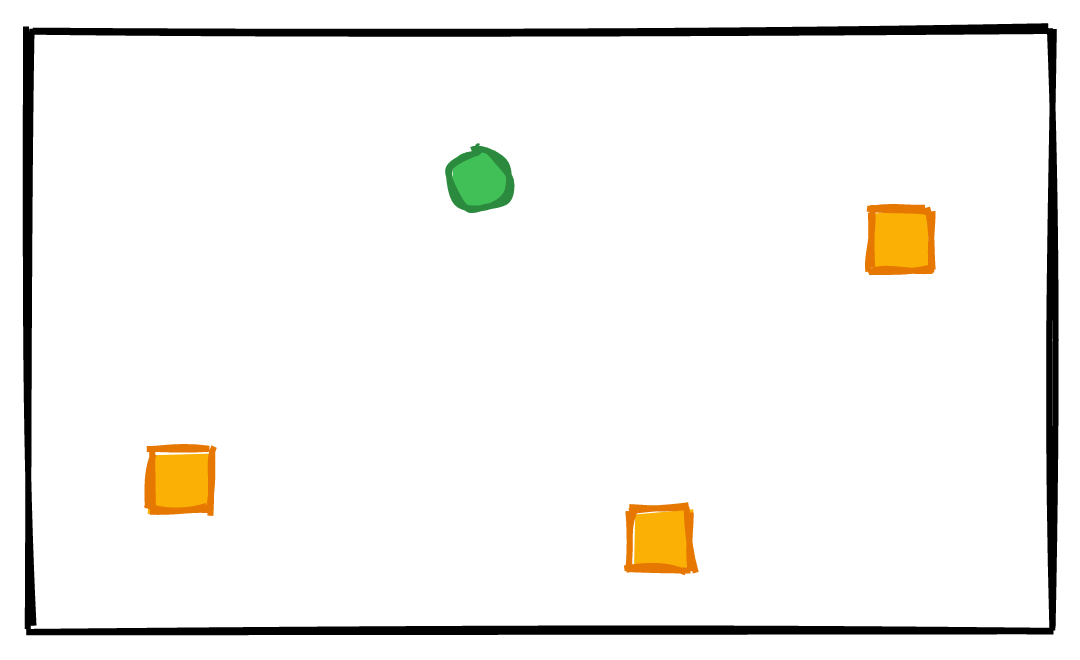
\includegraphics[width=0.9\textwidth]{figures/xrelation1.png}}%
            \only<2->{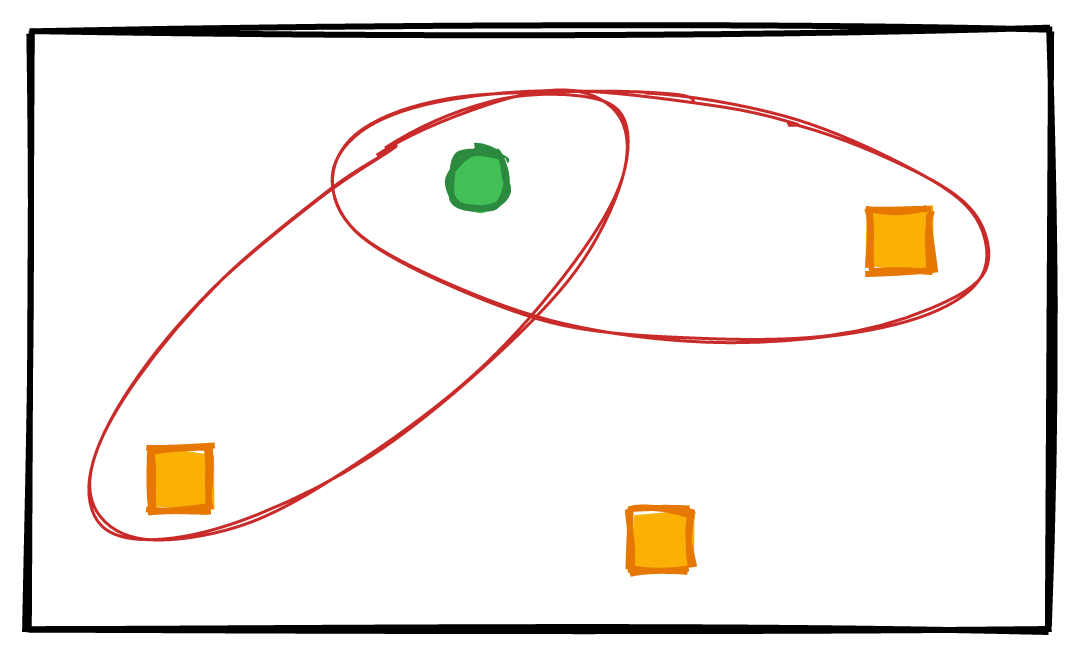
\includegraphics[width=0.9\textwidth]{figures/xrelation2.png}}
        \end{columns}
    \end{block}

    \begin{block}{Ideas:}
    \begin{enumerate}
        \small
        \item Sampled version of $\contMic_1,\contMic_2$ are available: $\discMic_1, \discMic_2$
        \item Echo TOAs $\propto$ sampling frequency
        \item Find echoes $\rightarrow$ \textbf{find sparse vectors} $\discRIR_1, \discRIR_2$ of length $L$
        \item Modeled as \textbf{Lasso}-like problem

        \vspace*{2mm}
        \begin{mysotablock}
            \begin{equation*}
                \widehat{\discRIR}_1, \widehat{\discRIR}_2 \in
                \underset{\discRIR_1, \discRIR_2\in\kR^n}{\arg\min}\;
                \Vert \discMic_1 \contConv \discRIR_2 - \discMic_2 \tikzmarknode{conv}{\contConv} \discRIR_1 \Vert_2^2
                + \lambda \mathcal{P}(\discRIR_1, \discRIR_2)
                \quad\text{s.t.}\quad\mathcal{C}(\discRIR_1, \discRIR_2)
            \end{equation*}

            \vspace*{-2mm}
            \begin{center}
                \footnotesize
                $\mathcal{P}(\discRIR_1, \discRIR_2)$ $\longrightarrow$ sparse promoting regularizer
                \hspace{5mm} \footnotesize $\mathcal{C}(\discRIR_1, \discRIR_2)$ $\longrightarrow$ constraints e.g. \parbox{6em}{nonnegativity\\anchor}
            \end{center}
        \end{mysotablock}
        \begin{tikzpicture}[overlay,remember picture, %
            nodes={inner sep=1pt, align=center, color=gray, font=\footnotesize}, %
            gray,>=stealth] %
            \draw[->] (conv.north) to[out=90, in=180] ++ (+10mm,+4mm) node[right] %
            {{= $\mathtt{Toeplitz}(\discMic_i) \discRIR_j \in \mathcal{O}(L^2)$}};
        \end{tikzpicture}
    \end{enumerate}
    \end{block}

    \vspace{-12mm}
    \begin{block}{}
        \begin{center}
            \footnotesize
            \textcolor{mygreen}{\cmark}  \cite{tong1994blind} \qquad \textcolor{mygreen}{\cmark}  \cite{lin2008blind} \qquad \textcolor{mygreen}{\cmark} \cite{aissa2008blind} \\
            \textcolor{mygreen}{\cmark} \cite{kowalczyk2013blind} \qquad \textcolor{mygreen}{\cmark} \cite{crocco2016estimation}
        \end{center}
    \end{block}

 \end{frame}


\begin{frame}{Proposed approach: analytical \& off-grid \hfill\faJediOrder}

    \begin{block}{\textbf{Observation 1:} the cross relation remains true in the frequency domain}
        \begin{equation*}
            \mathcal{F}x_1 \cdot \mathcal{F}h_2 (\sfrac{n}{F_s}) = \mathcal{F}x_2 \cdot \mathcal{F}h_1(\sfrac{n}{F_s}) \qquad n=0\dots N-1
        \end{equation*}
        \end{block}

        \vspace{.5em}

        \pause
        \begin{block}{\textbf{Observation 2:} $\mathcal{F}\delta_{\mathrm{echo}}$ is known in closed-form}
        \end{block}

        \pause
        \vspace{1.em}
        \begin{block}{\textbf{Observation 3:} $\mathcal{F}{\mathrm{x_i}}$ can be (well) approximated by DFT}
        \begin{equation*}
            \mathbf{X}_i = \texttt{DFT}(\discMic_i) \simeq  \mathcal{F}{\discMic_i}(nF_s) \qquad n=0\dots N-1
        \end{equation*}
        \end{block}


        \pause
        \vfill
        \setbeamercolor{block title}{fg=white,bg=darkblue}
        \setbeamercolor{block body}{fg=black,bg=bluegreen!10}
        \begin{block}{\textbf{Idea:} Recover echoes by matching a finite number of frequencies}
        \begin{equation*}
            \underset{h_1,h_2 \in \substack{\text{measure} \\ \text{space}}}{\arg\min} \;
            \tfrac{1}{2} \kvvbar{
                \mathbf{X}_1 \cdot \mathcal{F}h_2 (f) - \mathbf{X}_2 \cdot \mathcal{F}h_1(f)
            }_2^2
            + \lambda \kvvbar{h_1 + h_2}_{\mathrm{TV}}
            \quad
            \text{s.t.}\;
            \begin{cases}
                h_1(\{0\})=1 \\
                h_l \geq 0
                \end{cases}
        \end{equation*}
        \end{block}

        \pause
        \begin{center}
            $\sim$ \textbf{Lasso} problem, but $\mathcal{F}h_2 (f)$ is a continuous function.
            \\Instance of a \textbf{BLasso} problem~\cite{bredies2020sparsity}
            \\Solved with Sliding Frank-Wolfe algorithm \cite{denoyelle2019sliding}
        \end{center}

        \begin{center}
            \textcolor{mygreen}{\cmark{no Toeplitz matrix} \qquad
            \cmark \, \parbox{8.5em}{Solutions is \\ a train of Dirac} \qquad
            \cmark \, \parbox{8em}{anchor prevents \\ trivial solution}}
        \end{center}

        % In the manuscript:
        % \begin{itemize}
        %     \item From Lasso to BLasso
        %     \item Pseudocode of the Algorithm
        %     \item How to manually tuned lambda
        % \end{itemize}
\end{frame}

\begin{frame}[t]{\faFlask~Experimental results \hfill\faJediOrder}
    % \begin{block}{Scenario}
    %     \begin{itemize}
    %         \item simulation data with ISM with Pyroomacoustics
    %         \item 1 source, 2 microphones, random room geometry
    %         \item Full RIRs
    %         \item 2 sources: broadband and speech
    %         \item 2 datasets: different SNR, different RT60
    %     \end{itemize}
    % \end{block}
    \begin{columns}[onlytextwidth]
        \begin{column}{0.45\textwidth}
            \begin{block}{Methods}
                \begin{itemize}
                    \item BSN --- SIMO BCE\cite{lin2007blind}
                    \item IL1C: iteratively-weighted $\ell_1$ constraint SIMO BCE
                    \\\cite{crocco2015room}
                    \item \blaster: Proposed off-grid approach
                \end{itemize}
            Baseline method are xvalidated on other dataset
            \end{block}
        \end{column}

        \begin{column}{0.45\textwidth}
            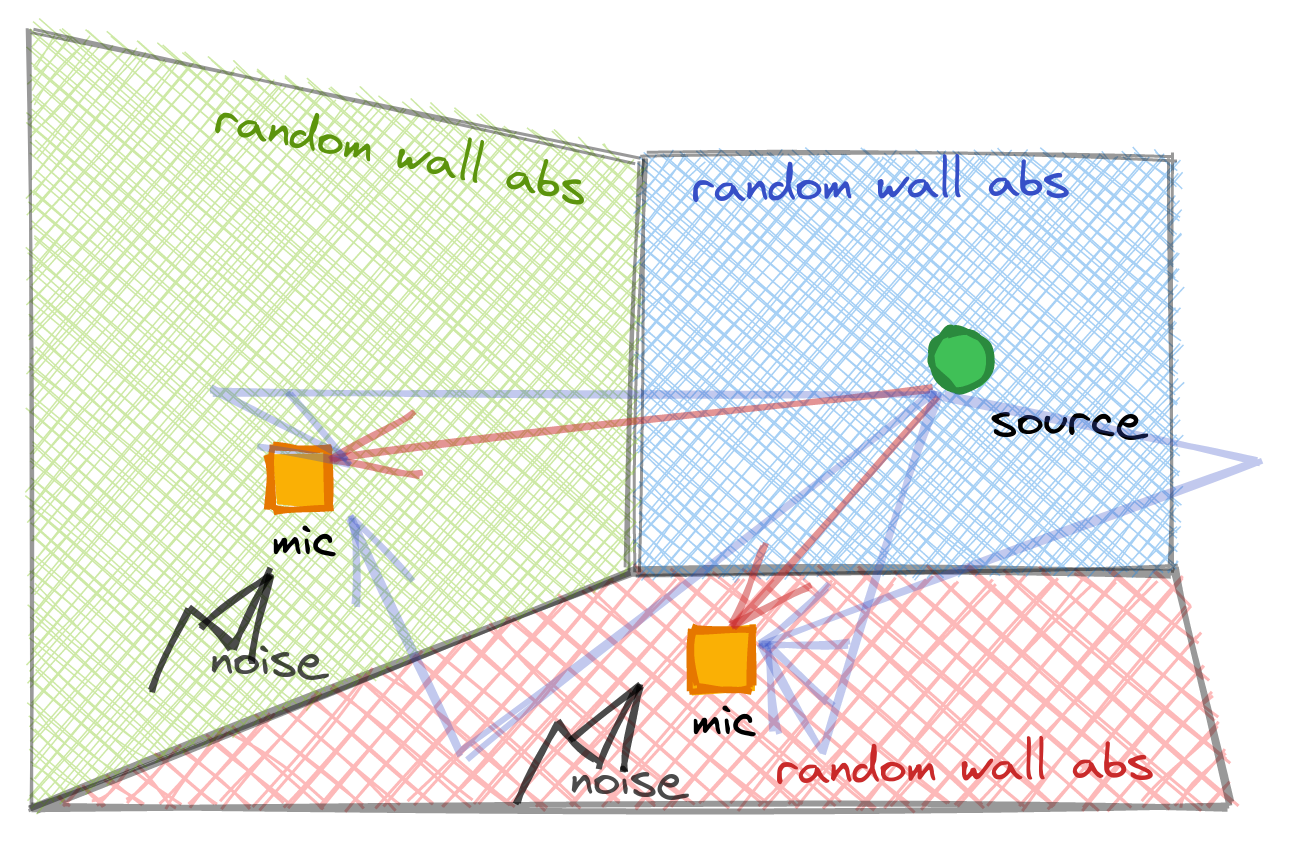
\includegraphics[width=0.9\textwidth]{figures/aer_scenario4.png}
        \end{column}
    \end{columns}

    \pause
    \begin{block}{Dataset}
        \begin{itemize}
            \footnotesize
            \item $\mathcal{D^{\text{SNR}}}$: $SNR \in [0, 20]$ dB, $\text{RT}_{60} = 400$ ms
            \item $\mathcal{D^{\text{RT60}}}$: $\text{RT}_{60} = [100, 1000]$ ms, $SNR = 20$ dB
        \end{itemize}
    \end{block}

    \pause
    \begin{block}{Metrics}
        \begin{itemize}
            \item Precision (how many estimated echoes are correct)
            \item RMSE (error on the correct guess)
        \end{itemize}
    \end{block}

\end{frame}


\begin{frame}<1>[label=echoes]{Performance per \# of echoes \hfill\faJediOrder}
    \begin{figure}[t!]
    \centering
        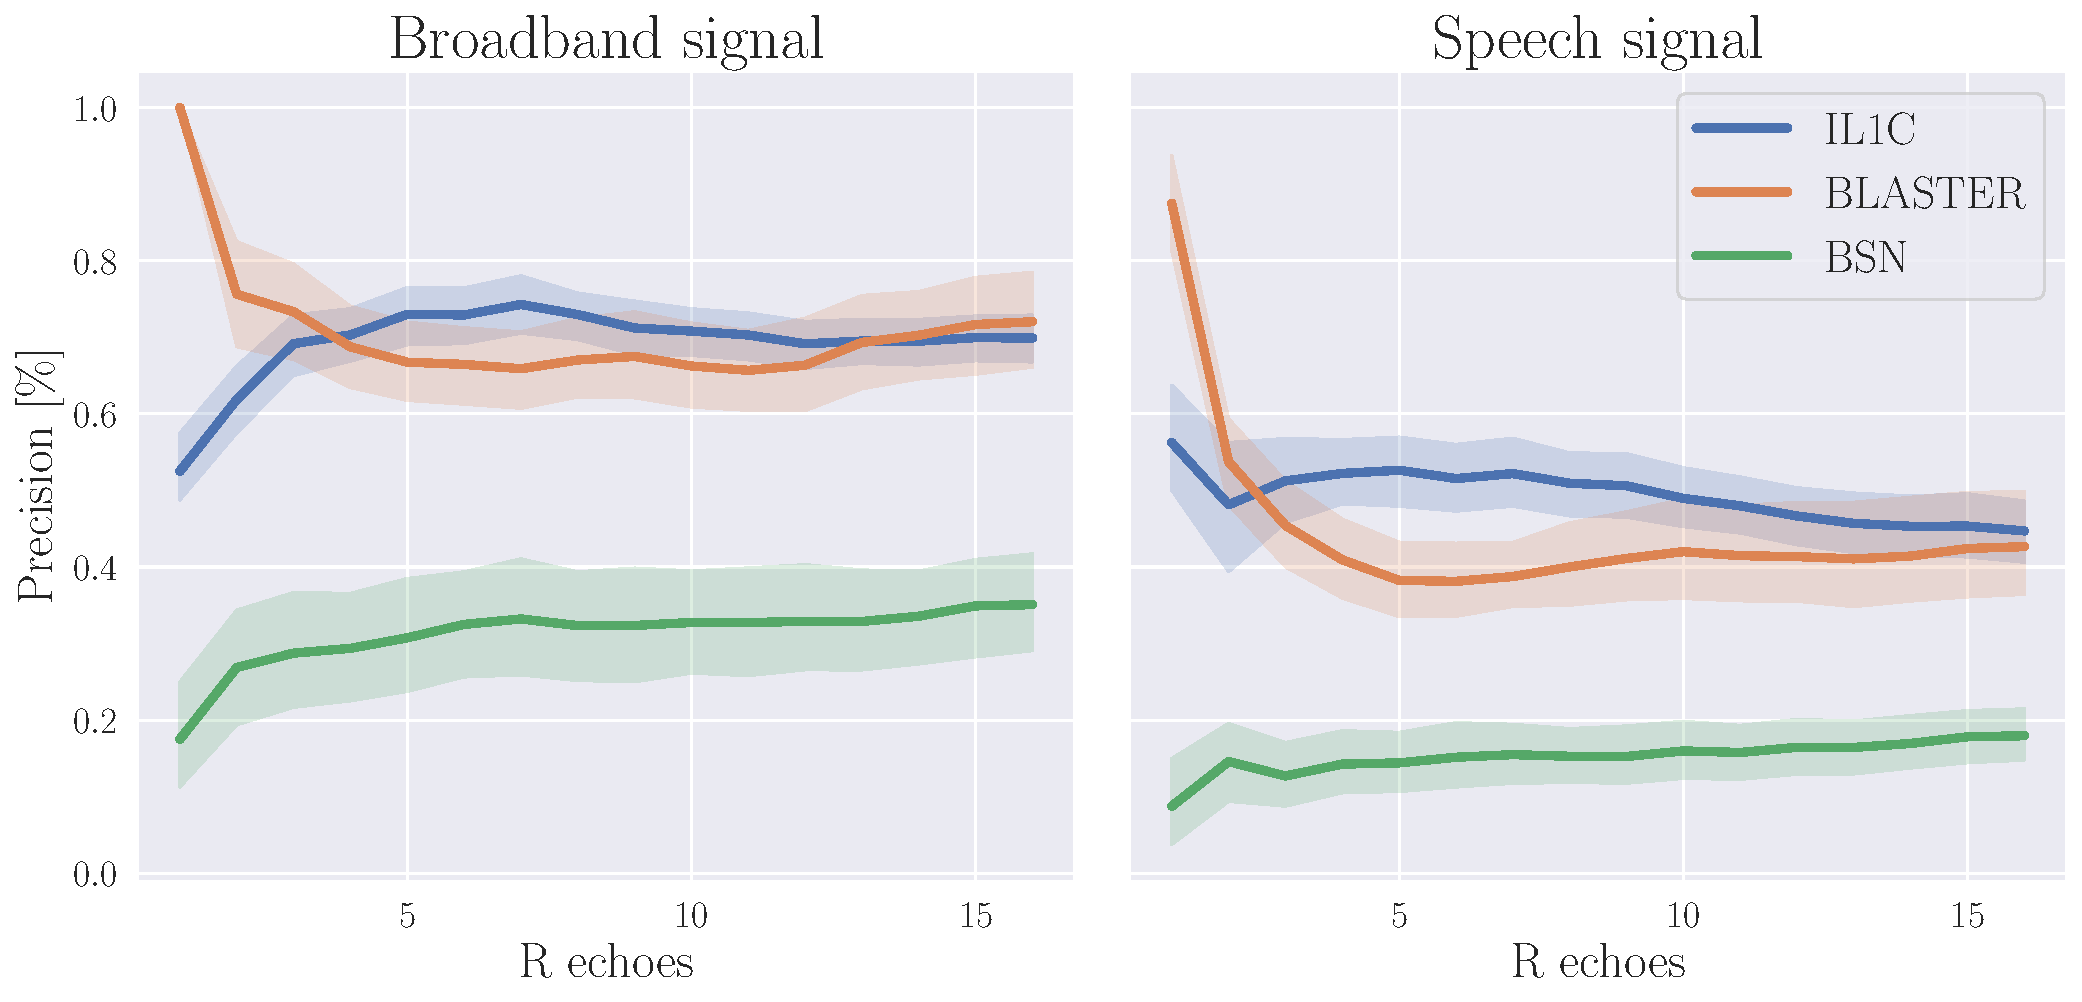
\includegraphics[width=\linewidth]{figures/p_k-7_thr-2_bns_crocco_blaster-peak_withRechoes.pdf}
        \caption{$\text{RT}_{60} = 400$ ms and SNR = 20 dB.}
    \end{figure}

    \begin{center}
        \textcolor{myred}{\xmark \: \parbox{8em}{Sensitive\\to \# echoes}}
        \textcolor{myred}{\xmark \: \parbox{8em}{Sensitive\\source signal}}
        \only<1>{
        \textcolor{mygreen}{\cmark \: \parbox{8em}{Good\\for 2 echoes}}
        }
        \only<2>{
        \textcolor{mygreen}{
        \cmark \: \parbox{8em}{Good\\for 2 echoes
                                    \\\cite{scheibler2018separake,di2019mirage}}}
        }
    \end{center}

\end{frame}

\againframe<2>{echoes}

\begin{frame}{Error per Dataset/Signal while recovering 7 echoes \hfill\faJediOrder}

    \begin{center}
        \begin{overpic}[width=0.8\textwidth]{figures/e_k-7_thr-2_bns_crocco_blaster.pdf}
            \put (102, 48){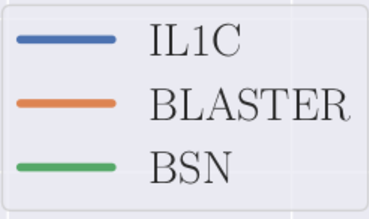
\includegraphics[width=5em]{figures/legend.pdf}}
        \end{overpic}
    \end{center}

    \begin{center}
        \textcolor{mygreen}{\cmark{Lower RMSE}} \qquad
        \textcolor{mygreen}{\cmark \, \parbox{8.5em}{Robustness\\
        to SNR and $\text{RT}_{60}$}} \qquad
        \textcolor{myred}{\xmark \, \parbox{8em}{Source signal\\dependent}}
    \end{center}

\end{frame}


% % \subsection{Interim conclusion (2/4)}

% % \begin{frame}{Interim conclusion (2/4)}
% %     \begin{block}{on Acoustic Echo Retrieval:}
% %         \begin{itemize}
% %             \item Most of the literature is on Passive and RIR-based, with on-grid approaches
% %             \item On-grid approaches suffers by the off-grid nature of the echoes (complexity, sampling)
% %         \end{itemize}
% %     \end{block}

% %     \begin{block}{on \blaster:}
% %         \begin{itemize}
% %             \item[\cmark] off-grid parameter-free which exploit dirac closed-form model (non negativity and sparsity)
% %             \item[\cmark] smaller RMSE due to super-resolution, better for small \# of echoes
% %             \item[\xmark] source dependent and on number of echoes
% %             \item[\xmark] validate only on synthetic data
% %             \item[$\rightarrow$] Multichannel and RTF-based extention
% %         \end{itemize}
% %     \end{block}

% %     \begin{block}{on \lantern:}
% %         \begin{itemize}
% %             \item[\cmark] promising results for first echo estimation
% %             \item[\cmark] direct application for table top application
% %             \item[\xmark] difficult extention
% %             \item[\xmark] need for real data validation
% %             \item[$\rightarrow$] physically-constrained neural network
% %             \item[$\rightarrow$] missing frequencies in the input
% %         \end{itemize}
% %     \end{block}
% % \end{frame}